\documentclass[tikz, border=10pt]{standalone}
\usetikzlibrary{shapes.geometric, arrows.meta, positioning, calc}

\begin{document}

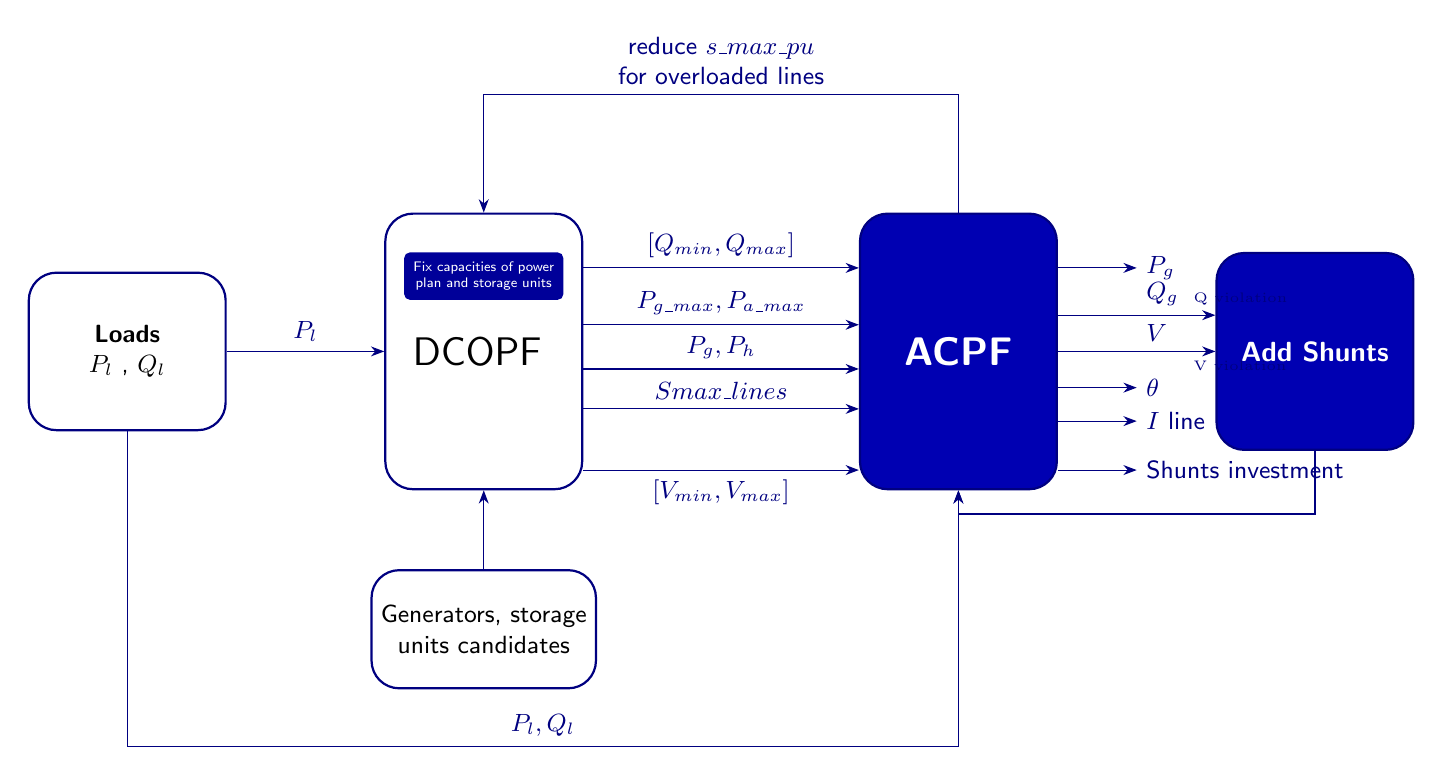
\begin{tikzpicture}[
    font=\sffamily\small,
    node distance=1.5cm and 2cm,
    >=Stealth,
    % Style des blocs
    block/.style={
        rectangle, 
        draw=blue!50!black, 
        fill=white, 
        rounded corners=10pt, 
        minimum width=2.5cm, 
        minimum height=3.5cm, 
        align=center,
        line width=0.8pt
    },
    blueblock/.style={
        block,
        fill=blue!70!black,
        text=white,
        font=\sffamily\Large\bfseries
    },
    innerblock/.style={
        rectangle,
        fill=blue!60!black,
        text=white,
        font=\sffamily\tiny,
        minimum width=2cm,
        rounded corners=2pt,
        align=center
    }
]

    % --- NŒUDS ---
    
    % Bloc de gauche : Loads
    \node[block, minimum height=2cm] (loads) { \textbf{Loads} \\ $P_l$ , $Q_l$ };

    % Bloc DCOPF
    \node[block, right=of loads] (dcopf) { \Large DCOPF };
    % Petit bloc bleu à l'intérieur du DCOPF
    \node[innerblock, anchor=north, yshift=-0.5cm] at (dcopf.north) {Fix capacities of power\\plan and storage units};

    % Bloc ACPF
    \node[blueblock, right=3.5cm of dcopf] (acpf) {ACPF};

    % Bloc Add Shunts
    \node[blueblock, right=2cm of acpf, minimum height=2.5cm, font=\sffamily\bfseries] (shunts) {Add Shunts};

    % Bloc Generators en bas
    \node[block, below=1cm of dcopf, minimum height=1.5cm] (gen) {Generators, storage\\units candidates};

    % --- LIAISONS / FLÈCHES ---

    % Loads -> DCOPF
    \draw[->, blue!50!black] (loads) -- node[above] {$P_l$} (dcopf);

    % Loads -> ACPF (Ligne coudée en bas)
    \draw[->, blue!50!black] (loads.south) -- ++(0,-4) -| node[pos=0.25, above] {$P_l, Q_l$} (acpf.south);

    % Gen -> DCOPF
    \draw[->, blue!50!black] (gen) -- (dcopf);

    % DCOPF -> ACPF (Multiples flèches avec étiquettes)
    \begin{scope}[every edge/.style={draw, ->, blue!50!black}]
        \path (dcopf.40)  edge node[above] {$[Q_{min}, Q_{max}]$} (acpf.140);
        \path (dcopf.15)  edge node[above] {$P_{g\_max}, P_{a\_max}$} (acpf.165);
        \path (dcopf.-10) edge node[above] {$P_g, P_h$} (acpf.190);
        \path (dcopf.-30) edge node[above] {$Smax\_lines$} (acpf.210);
        \path (dcopf.-50) edge node[below] {$[V_{min}, V_{max}]$} (acpf.230);
    \end{scope}

    % ACPF -> DCOPF (Boucle retour en haut)
    \draw[->, blue!50!black] (acpf.north) -- ++(0,1.5) -| node[pos=0.25, above, align=center] {reduce $s\_max\_pu$ \\ for overloaded lines} (dcopf.north);

    % ACPF -> Add Shunts (Sorties)
    \path[->, blue!50!black] (acpf.20)  edge node[above right] {$Q_g$} node[pos=0.8, anchor=south west, font=\tiny] {Q violation} (shunts.160);
    \path[->, blue!50!black] (acpf.0) edge node[above right] {$V$} node[pos=0.8, anchor=north west, font=\tiny] {V violation} (shunts.180);
    

    % Autres sorties de l'ACPF vers le vide (comme sur l'image)
    \draw[->, blue!50!black] (acpf.40)  -- ++(1,0) node[right] {$P_g$};
    \draw[->, blue!50!black] (acpf.-20) -- ++(1,0) node[right] {$\theta$};
    \draw[->, blue!50!black] (acpf.-35) -- ++(1,0) node[right] {$I$ line};
    \draw[->, blue!50!black] (acpf.-50) -- ++(1,0) node[right] {Shunts investment};

    % Add Shunts -> ACPF (Boucle retour en bas)
    \draw[->, blue!50!black] (shunts.south) -- ++(0,-0.8) -| (acpf.south);

\end{tikzpicture}

\end{document}